\chapter{Lecture 26 - Laplace's Equation}
\label{ch:lec26}
\section{Objectives}
\begin{itemize}
\item Solve an example problem with solution for Laplace's equation representing steady-state temperature in a rectangular domain.
\item Show how to use the superposition principle to solve Laplace's equation with multiple non-homogeneous boundary conditions.
\end{itemize}
\setcounter{lstannotation}{0} %hack to try and re-set annotation counter.

\section{Laplace Equation Example}
Consider the system depicted in Figure \ref{fig:lec26-fig1} and described by the following boundary value problem based on Laplace's Equation.
\begin{marginfigure}
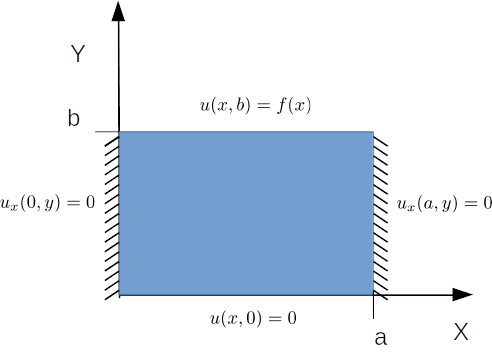
\includegraphics{lec26_fig1.png}
\caption{Schematic of example Laplace's equation problem.}
\label{fig:lec26-fig1}
\end{marginfigure}
\begin{table}[h]
\begin{tabular}{l l}
$\substack{\text{Governing} \\\text{Equation}}: $& $\frac{\partial^2 u}{\partial x^2} + \frac{\partial^2 u}{\partial y^2} = 0, \ \ 0<x<a, \ \ 0<y<b $\\
& \\
$\substack{\text{Boundary} \\ \text{Conditions}}: $ & $\substack{u(x,0)=0  \ \ \ \ \ \ u_x(0,y) = 0 \\ \\ u(x,b) = f(x) \ \ u_x(a,y) = 0}$ 
\end{tabular}
\end{table} 
We will find the solution to this boundary value problem using separation of variables.

\vspace{0.25cm}

\noindent\textbf{Step \#1:} Assume a product solution.
\begin{equation*}
u(x,y) = F(x)G(y)
\end{equation*}

\vspace{0.25cm}

\noindent\textbf{Step \#2:} Insert proposed solution into the governing equation.

\begin{align*}
\frac{\partial^2}{\partial x^2}\left(F(x)G(y)\right) + \frac{\partial^2}{\partial y^2}\left(F(x)G(y)\right) &= 0 \\
F_{xx}G + FG_{yy} &= 0
\end{align*}

\vspace{4.5cm}

\noindent\textbf{Step \#3:} Separate variables by dividing by $F(x)G(y)$:\marginnote{Once again we assume that neither $F(x)$ nor $G(y)$ are identically equal to zero throughout the domain, therefore it is mathematically acceptable for them to appear in the denominator.}
\begin{align*}
\frac{F_{xx}G}{FG} + \frac{FG_{yy}}{FG} &= 0 \\
\frac{F_{xx}}{F} + \frac{G_{yy}}{G} &= 0 \\
\frac{F_{xx}}{F} = -\frac{G_{yy}}{G} &= -\lambda \\
F_{xx}+\lambda F &= 0 \\
G_{yy}-\lambda G &= 0
\end{align*}
This gives us two separated boundary value problems to solve.

\vspace{0.5cm}

\noindent\textbf{Step \#4:} Apply boundary conditions to determine non-trivial product solution(s)
\begin{marginfigure}
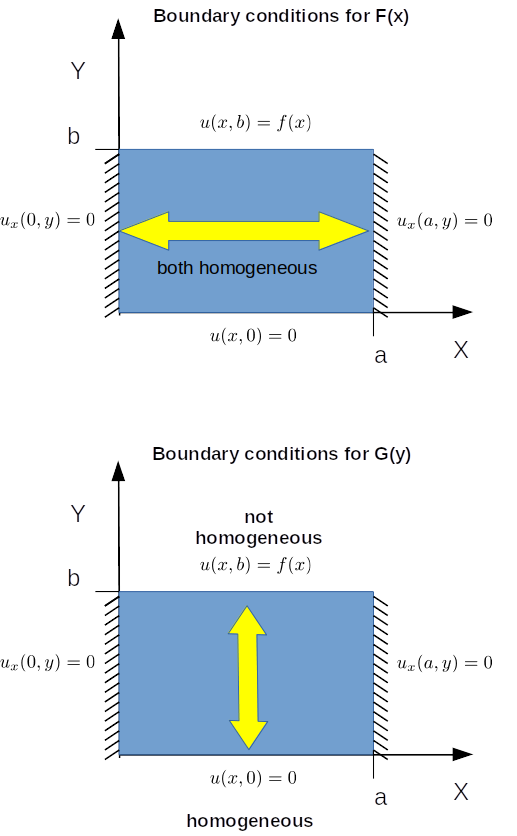
\includegraphics{lec26_bcs.png}
\caption{Pairs of boundary conditions for Laplace's equation.}
\label{fig:lec26-bcs}
\end{marginfigure}

\vspace{0.1cm}

\noindent In order to determine allowable values for $\lambda$, we find solutions to the separated boundary value problem that has \emph{all homogeneous boundary conditions.}  So we will examine $F_{xx} + \lambda F = 0$.  As usual, we will have to check for all possible values of $\lambda$.

\vspace{0.1cm}

\noindent\underline{$\lambda = 0$}:

\begin{align*}
F_{xx} &= 0 \\
F(x) &= c_1x + c_2 \\
\Rightarrow F_{x} &= c_1 \\
F_x(0) = c_1 &= 0 \\ 
F_{x}(a) &= 0 \ \text{ (satisfied)}
\end{align*}

\vspace{0.1cm}

\noindent We see that, while $c_1$ must be zero, $F(x)=c_2$ satisfies both boundary conditions for any value of $c_2$.  Thus $\lambda = 0$ is an acceptable eigenvalue.

\vspace{0.1cm}

\noindent\underline{$\lambda < 0$}:
